\documentclass[letterpaper,10pt]{article}

\usepackage{titling}
\usepackage{listings}
\usepackage{url}
\usepackage{setspace}
\usepackage{subfig}
\usepackage{sectsty}
\usepackage{pdfpages}
\usepackage{colortbl}
\usepackage{multirow}
\usepackage{relsize}
\usepackage{amsmath}
\usepackage{fancyvrb}
\usepackage{amsmath,amssymb,amsthm,graphicx,xspace}
\usepackage[titlenotnumbered,noend,noline]{algorithm2e}
\usepackage[compact]{titlesec}
\usepackage{paratype} 
\usepackage[T1]{fontenc}
\usepackage{tikz}
\usetikzlibrary{arrows,automata,shapes,trees,matrix,chains,scopes,positioning,calc}
\tikzstyle{block} = [rectangle, draw, fill=blue!20, 
    text width=2.5em, text centered, rounded corners, minimum height=2em]
\tikzstyle{bw} = [rectangle, draw, fill=blue!20, 
    text width=4em, text centered, rounded corners, minimum height=2em]

\definecolor{namerow}{cmyk}{.40,.40,.40,.40}
\definecolor{namecol}{cmyk}{.40,.40,.40,.40}

\let\LaTeXtitle\title
\renewcommand{\title}[1]{\LaTeXtitle{\textsf{#1}}}


\newcommand{\handout}[5]{
  \noindent
  \begin{center}
  \framebox{
    \vbox{
      \hbox to 5.78in { {\bf ECE254: Operating Systems and Systems Programming } \hfill #2 }
      \vspace{4mm}
      \hbox to 5.78in { {\Large \hfill #4  \hfill} }
      \vspace{2mm}
      \hbox to 5.78in { {\em #3 \hfill} }
    }
  }
  \end{center}
  \vspace*{4mm}
}

\newcommand{\lecture}[3]{\handout{#1}{#2}{#3}{Lecture #1}}
\newcommand{\tuple}[1]{\ensuremath{\left\langle #1 \right\rangle}\xspace}

\addtolength{\oddsidemargin}{-1.000in}
\addtolength{\evensidemargin}{-0.500in}
\addtolength{\textwidth}{2.0in}
\addtolength{\topmargin}{-1.000in}
\addtolength{\textheight}{1.75in}
\addtolength{\parskip}{\baselineskip}
\setlength{\parindent}{0in}
\renewcommand{\baselinestretch}{1.5}
\newcommand{\term}{Spring 2015}

\singlespace


\begin{document}

\lecture{ 25 --- Uniprocessor Scheduling }{\term}{Jeff Zarnett}

\section*{Uniprocessor Scheduling}

As you may imagine, processor scheduling can be very complex when we have multiple processes and multiple processors. Accordingly, to keep things simple, we will start with single processor systems (uniprocessor scheduling) and then build on that to look into multiprocessor scheduling.

Scheduling is easy to define: given that we have multiple processes in the system, we are going to have to make some decisions about when different programs run. There are four types of scheduling, but one of the four is I/O scheduling which we will come back to later on. The other three bear more examination~\cite{osi}:

\begin{enumerate}
	\item \textbf{Long-Term Scheduling}
	\item \textbf{Medium-Term Scheduling}
	\item \textbf{Short Term Scheduling}
\end{enumerate}

A student-relevant analogy to explain the different levels: Long-term scheduling is deciding what courses to take in your degree (e.g., do I want to take ECON~102 as a non-technical elective?). Medium-term scheduling is about deciding what courses you are taking in a given term (do I take ECON~102 in 2B or 4A?). Short term scheduling is deciding what course you are going to study right now (I'll study ECE~254 because the final exam is tomorrow!)

\paragraph{Long-Term Scheduling.}

The long term scheduler is responsible for determining which programs are going to run at all. It controls how many jobs the system is accepting to do at once. It controls the transition from the ``new'' state into the ready to run state (where it falls in the purview of the medium or short term scheduler). When a process exits, the long term scheduler might decide to admit a new one. Ah, but which one! The first? Based on some criteria?

Long term scheduling does not tend to happen too much on desktop computer systems. The user controls how many processes are running at a given time. If you choose to open 50 programs, performance may suffer, but the OS will not attempt to stop you.

Mind you, in rare occasions, there is some form of long term scheduling. If you are trying to log into a server, because you want to play Diablo III\footnote{Barbarian, for the curious.}, you may receive an error saying the server is busy/full. This is the server telling you that it will not start a new game for you (a new process) because it has reached a limit of how many processes (games) are currently permitted. Only when some people log out will you be allowed to log in.

Mobile operating systems, notably Android, can be somewhat more aggressive. If memory is running low, Android can suspend and kill processes to make way for new ones.

\paragraph{Medium-Term Scheduling.}
Medium term scheduling is a lot more interesting than long term scheduling, and it revolves around swapping processes to and from disk. A process that is swapped to disk is not going to run in the immediate future, but it is at least likely to run before too long. Swapping a process to disk takes it out of the realm of the short term scheduler; swapping it in to memory returns it to that domain.

\paragraph{Short-Term Scheduling.}
The short term scheduler, also sometimes called the dispatcher, is where the real action is. The medium and long term scheduler are all about someday and sometime and whenever. The short term scheduler is about ``what are we going to do \textit{right now}''. The short term scheduler is going to run a lot, so it is very important. The short term scheduler will often run after certain things occur. 

If we have co-operative multitasking, short term scheduling will only take place in one of two circumstances: the currently executing process yields the CPU or the currently executing process terminates (voluntarily or with an error). This is not how most operating systems work these days (though Mac OS 9 did follow this scheme, fortunately, its successor of Mac OS X does not). If the process does yield or terminate, then the short term scheduler will run.

For reasons that are presumably obvious (hint: some people are jerks), co-operative multitasking is problematic. What we will discuss from here on out is pre-emptive multitasking; the operating system, and not the running process, is responsible for deciding when it's time to switch processes. Some pre-emptive systems still have the concept of yield, and that is still an occasion to run the scheduler. Similarly, in pre-emptive systems, processes still terminate.

The dispatcher will certainly run when a process becomes blocked, such as on an I/O operation. If a process requested a write to the network and is blocked, now the short term scheduler needs to decide what process runs next. If it gets blocked on a semaphore or mutex, that is also an occasion to switch to another process. Page faults are also a great occasion to find something else to do.

Another time to make a scheduling decision is after handling an interrupt, whether from an I/O device or otherwise. After the interrupt is handled, we can return to execution exactly where we left off, or we can go somewhere else (the original process is suspended already so why not leave it in that state?). 

System calls like \texttt{fork} and even signalling on a semaphore may also provide good opportunities to switch from one process to another. Again, by invoking the operating system through the system call, the calling process is suspended (the trap handler runs and the OS takes over). So it is necessary to decide what process executes next. We acknowledged this in the discussion of \texttt{fork} by saying it was not known if the parent or child would execute next. In the case of semaphores, we do not even know which of the processes waiting on the semaphore will be the one to receive the signal, and even then, which of the signalling process and waiting process will resume.

Finally, there is also time slicing. If time slices are defined as $t$ units, every $t$ time units, there will be an interrupt generated by the clock. The whole purpose of the interrupt handler in that case is to run the short term scheduler to choose a process to run, so that different processes run (seemingly-)concurrently.

\subsection*{Process Behaviour: Rate Limiting Step}

Processes tend to alternate periods of computing with input/output requests. These tend to alternate, so for a while the CPU does a lot of work, called a \textit{CPU Burst}, and then it needs to do some I/O, and the period where it is waiting is called the \textit{I/O Burst}. After the I/O is completed, the CPU can go at it again. How much of each a process does allows for classification of the process into one of two categories.

Processes that spend most of their time computing are called \textit{CPU-Bound} and the limiting factor in their execution is how fast the CPU executes the code. Complex mathematical equations, for example, require a lot of CPU time. They can speed up significantly if you get a faster CPU. The alternative is a process that spends most of its time waiting for I/O, which we call \textit{I/O Bound}. In this case, having a faster CPU will not make the difference in how long it takes to execute the program. See the diagram below:

\begin{center}
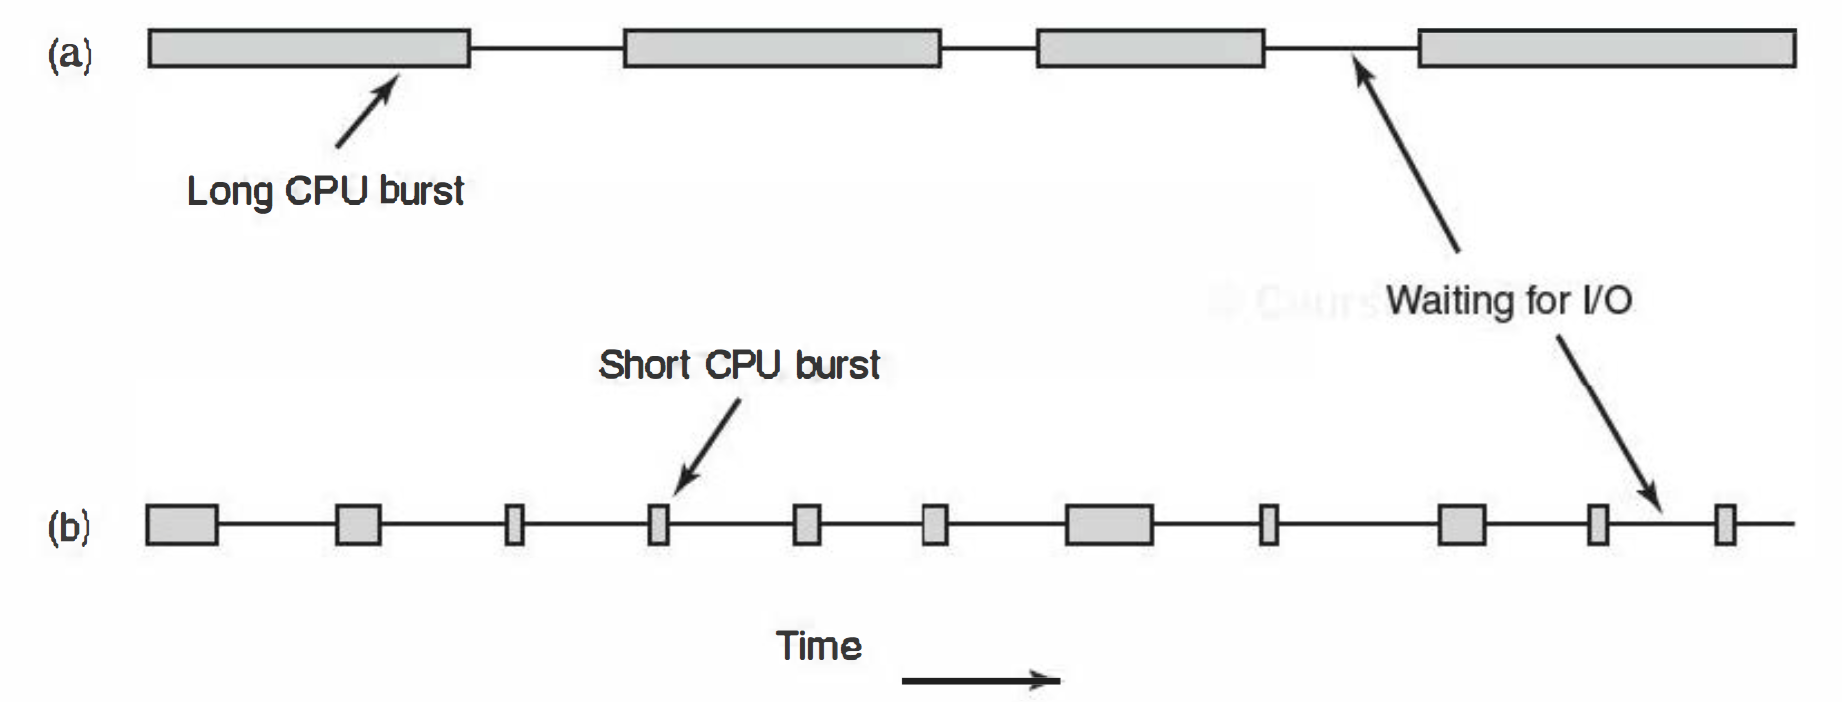
\includegraphics[width=0.75\textwidth]{images/cpu-io-bound.png}\\
CPU usage diagram showing (a) a CPU-Bound process and (b) an I/O-Bound process~\cite{mos}.
\end{center}

Studies have been done to examinee the durations of CPU bursts. An I/O bound program will tend to have short CPU bursts, of course. Over time, CPUs have gotten faster at a rate much higher than the rate of I/O speedup. This is probably not surprising to you: a new CPU comes out every few months and they get faster. I/O standards like Serial-ATA and USB and such change very slowly, over the course of years. So it makes sense that over time programs tend towards being I/O bound. The results of the study are shown below:

\begin{center}
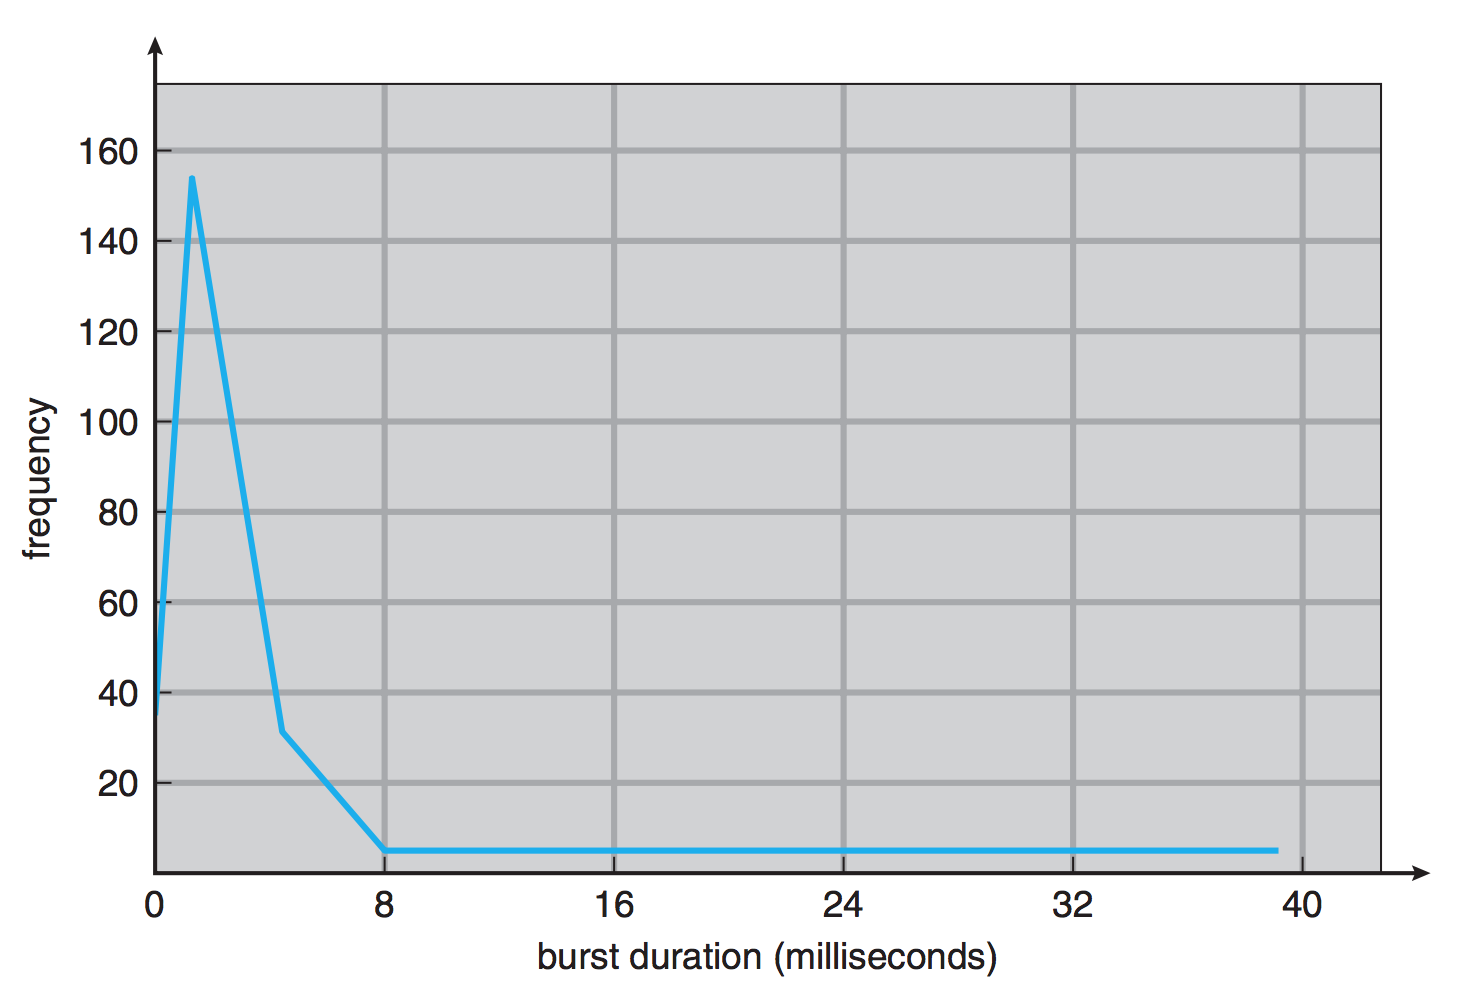
\includegraphics[width=0.65\textwidth]{images/cpu-burst-histogram.png}\\
CPU-Burst histogram~\cite{osc}.
\end{center}

But what does this have to do with scheduling? There are two applications. The long term scheduler may attempt to keep a balance between CPU- and I/O-bound tasks to get the best resource utilization. This requires that the long term scheduler have some idea about which processes are which.

Another is that if the disk is a common ``pinch point'', when the disk has nothing to do, the short term scheduler should immediately schedule a process that is likely to issue a disk request, so the disk is kept as busy as possible.

\subsection*{Scheduling Criteria}

The goals of scheduling depend significantly on the objectives of the system. If the system is supposed to respond to events within a certain period of time (real time system), this matters a lot to scheduling. Perhaps the goal is for the CPU to be used maximally (as in a supercomputer). Or maybe the most important thing is for users to feel like the system answers them quickly when they issue a command.

As usual when making a decision, we could just decide randomly. You may safely assume that just picking at random is not going to do well. So we should make an intelligent decision and  we therefore need evaluation criteria.

We will examine the following scheduling criteria~\cite{osi}:

\begin{enumerate}
	\item Turnaround time.
	\item Response time.
	\item Deadlines.
	\item Predictability.
	\item Throughput.
	\item Processor utilization.
	\item Fairness.
	\item Enforcing priorities.
	\item Balancing resources.
\end{enumerate}

\paragraph{Turnaround Time.} The turnaround time is the amount of time between starting a process and when it finishes. This is the execution time plus the amount of time waiting for resources (processor, I/O, etc). So, wall-clock time matters here. This is important to users; all things being equal the users would like their task to complete as fast as possible. If I ask the system to convert a file from FLAC format to mp3 format so I can import it to my mp3 player, I care about the turnaround time: how long will it take to convert this file?

\paragraph{Response Time.} Assuming a process is not a background process (daemon), this is the time between putting in a request and getting some answers back. A process can often start producing output while still doing the request. If I am searching for a file on disk, while the search continues to run, any results found so far can be shown in the results list. Response time is very important to users; if they click a button and it takes a long time to acknowledge the command, users get frustrated and sometimes issue the command more than once. Like the time I accidentally bought two train tickets via an Android app\footnote{Fortunately, this was a single ride ticket, so it was only a 5 Euro mistake and not a monthly ticket which could have easily been a 100+ Euro mistake.}.

\paragraph{Deadlines.} This is more of a concern for real-time systems that have specific deadlines. If I am watching a movie with a Blu-Ray player, the player needs to read data from the disk, decrypt and decode it, and display it to the screen within a certain period of time, otherwise the video quality is degraded. Meeting the deadlines may be the most important thing in the system; much depends on the application.

\paragraph{Predictability.} It is desirable if a given job runs in a fairly consistent amount of time. If a task normally takes $x$ minutes and right now it is taking $2x$ minutes, somewhere between $x$ and $2x$ minutes, the user may fear the process is stuck and might terminate it. Users are very impatient.

\paragraph{Throughput.} Scheduling policy should try to maximize the number of processes that complete in a given amount of time. This is our way of figuring out how much work is being accomplished. Much will depend here on the nature of the processes, but we would always like to get more done in the same amount of time. If I am in line to renew my drivers' license, if the Service Ontario office has a high throughput, more people will get their requests finished in the day. If it has a low throughput, I may be waiting there all day. Which would never happen. Oh no.

\paragraph{Processor Utilization.} This is, obviously, how much of the time the CPU is busy. As already mentioned, supercomputers are really expensive to build and maintain. Processing time on supercomputers is sold (leased?) to various organizations like research labs and universities. Any time the supercomputer is not in use is wasted. So we may give a lot of priority to keeping it busy.

\paragraph{Fairness.} Who could be against fairness? Humans have a lot of inbuilt notions about fairness, but we are not necessarily expecting a perfectly fair routine for scheduling. What we do expect, however, is that processes should get at least a basic level of fairness, e.g., no starvation. There is a story, possibly apocryphal, about a system being shut down in 1972 that had a yet-unexecuted batch job that had been submitted some five years earlier. I think we can safely call that unfair.

\paragraph{Priorities.} Processes can be assigned priorities: a way of saying that this process is more or less important compared to others. Scheduling should respect this, within reasonable limits. The highest priority process should probably run most often, but it should not always be the one selected, as that would violate the principle of fairness.

\paragraph{Balancing Resources.} We will get a better outcome if we balance resource usage. The example mentioned about applies: we would like to choose some CPU-Bound and I/O-Bound processes so both the CPU and I/O are kept busy. If we have more information about what sort of I/O the processes will need, so much the better: we can choose a process that will use the printer if run, when we know the printer is idle, and avoid choosing a process that will use the network if we know the network is busy.

\subsubsection*{Scheduling Algorithm Goals}

The priorities of these different goals depend significantly on the kind of system it is. The following list gives some idea about what is important in different kinds of systems~\cite{mos}:

\paragraph{All Systems.}
\begin{itemize}
	\item Fairness
	\item Priorities
	\item Balancing Resources
\end{itemize}

\paragraph{Batch Systems.}
\begin{itemize}
	\item Throughput
	\item Turnaround time
	\item CPU Utilization
\end{itemize}

\paragraph{Interactive Systems.}
\begin{itemize}
	\item Response time.
	\item Predictability.
\end{itemize}

\subsection*{The (Ab)use of Priorities}

Okay, so we've said that processes have priorities and we've repeatedly references priority as being an important consideration in various operations like scheduling and page allocation and so on. We have not yet actually talked much about priorities.

Each process's priority is typically an integer. Whether higher numbers are higher priority or lower numbers are higher priority is a question of system design. As is typical, if there are two ways to do something, some people will choose one way and some will choose the other. In UNIX, a lower number is higher priority; Windows is the opposite. Picking a convention and sticking to it would be nice, but there we are.

With a priority value assigned, it can be used to make decisions about resources. If $P_{1}$ wants resource $R_{1}$ and $P_{2}$ wants that same resource, where the priority of $P_{1}$ is greater than that of $P_{2}$, choose to assign the resource to $P_{1}$.

The operating system or the program author may be responsible for assigning a priority to each of the processes. These priorities may change over time with various criteria. System administrators can change priorities, usually.

Users may have a say in priority, in at least a limited way. In Windows, for example, as a user it may be possible to set a task to a higher or lower priority. Giving this to users was probably a bad idea, because users often do it wrong. If you have a long, CPU-Bound task, the right thing to do is to give it a low priority and not a high one. You might expect that the high priority will get the task done faster, but it kills the performance of the system and makes users unhappy (even though that's what they wanted).

In some systems, the highest priority non-blocked process will always run. This is a great way of making sure that higher priority processes have right-of-way, but a terrible way of ensuring fairness and preventing starvation. We could easily have a situation where low priority processes never get a chance to run, because there are too many processes of middle or high priority. So, scheduling is not necessarily as easy as just finding the highest priority thing to do...


\bibliographystyle{alpha}
\bibliography{254}


\end{document}